\documentclass{beamer}

\usepackage{graphicx}

\title{Week 1 CUSF Controls Freshers Project - Introduction}
\author{Yoonjae Hwang}
\date{12 October 2025}

\begin{document}

\frame{\titlepage} 

\begin{frame}
\frametitle{Motivation}
\begin{itemize}
    \item Spacecrafts are highly complex systems
    \item Disturbances are everywhere and we can't predict everything that will happen
    \item We need a way to automatically correct the motion of the spacecraft against disturbances
    \item Lower level control systems will be present all throughout the system of the spacecraft
    \item Control systems use feedback
\end{itemize}
\end{frame}

\begin{frame}
\frametitle{What is Feedback?}
\begin{center}
    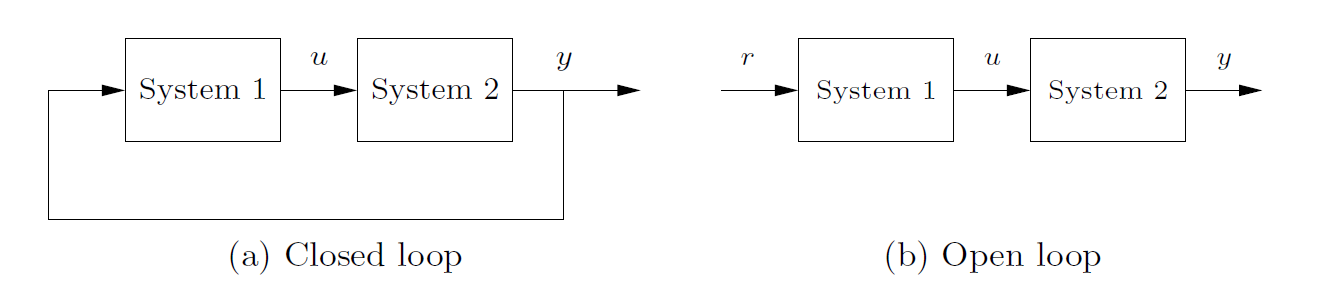
\includegraphics[width=0.7\textwidth]{closedloop.png}
\end{center}
\begin{itemize}
    \item Dynamical systems are systems whose behaviour change with time
    \item External forces or Disturbances
    \item Systems takes inputs and produces outputs
    \item Feedback is when the output of the system affects the input
    \item Control theory is a subject developed to formally approach the study of feedback
    \item Closed loop: Systems with feedback
    \item Open loop: Systems without feedback
\end{itemize}
\end{frame}

\begin{frame}
\frametitle{Feedforward?}
\begin{itemize}
    \item Feedback is reactive
    \item Feedforward measures disturbances before it enters a system
    \item Informs corrective action before the disturbance affects the system
\end{itemize}
\end{frame}

\begin{frame}
\frametitle{What is Control?}
\begin{columns}
\begin{column}{0.5\textwidth}
\begin{itemize}
    \item Use of feedback and algorithms to change an engineering system to a desired state
    \item Performance
    \item Stability
    \item Guarantees
    \item Robustness to uncertainty and disturbances
    \item Sensors
    \item Implementation happens through software onto microcontrollers, with C or C++
\end{itemize}
\end{column}

\begin{column}{0.5\textwidth}
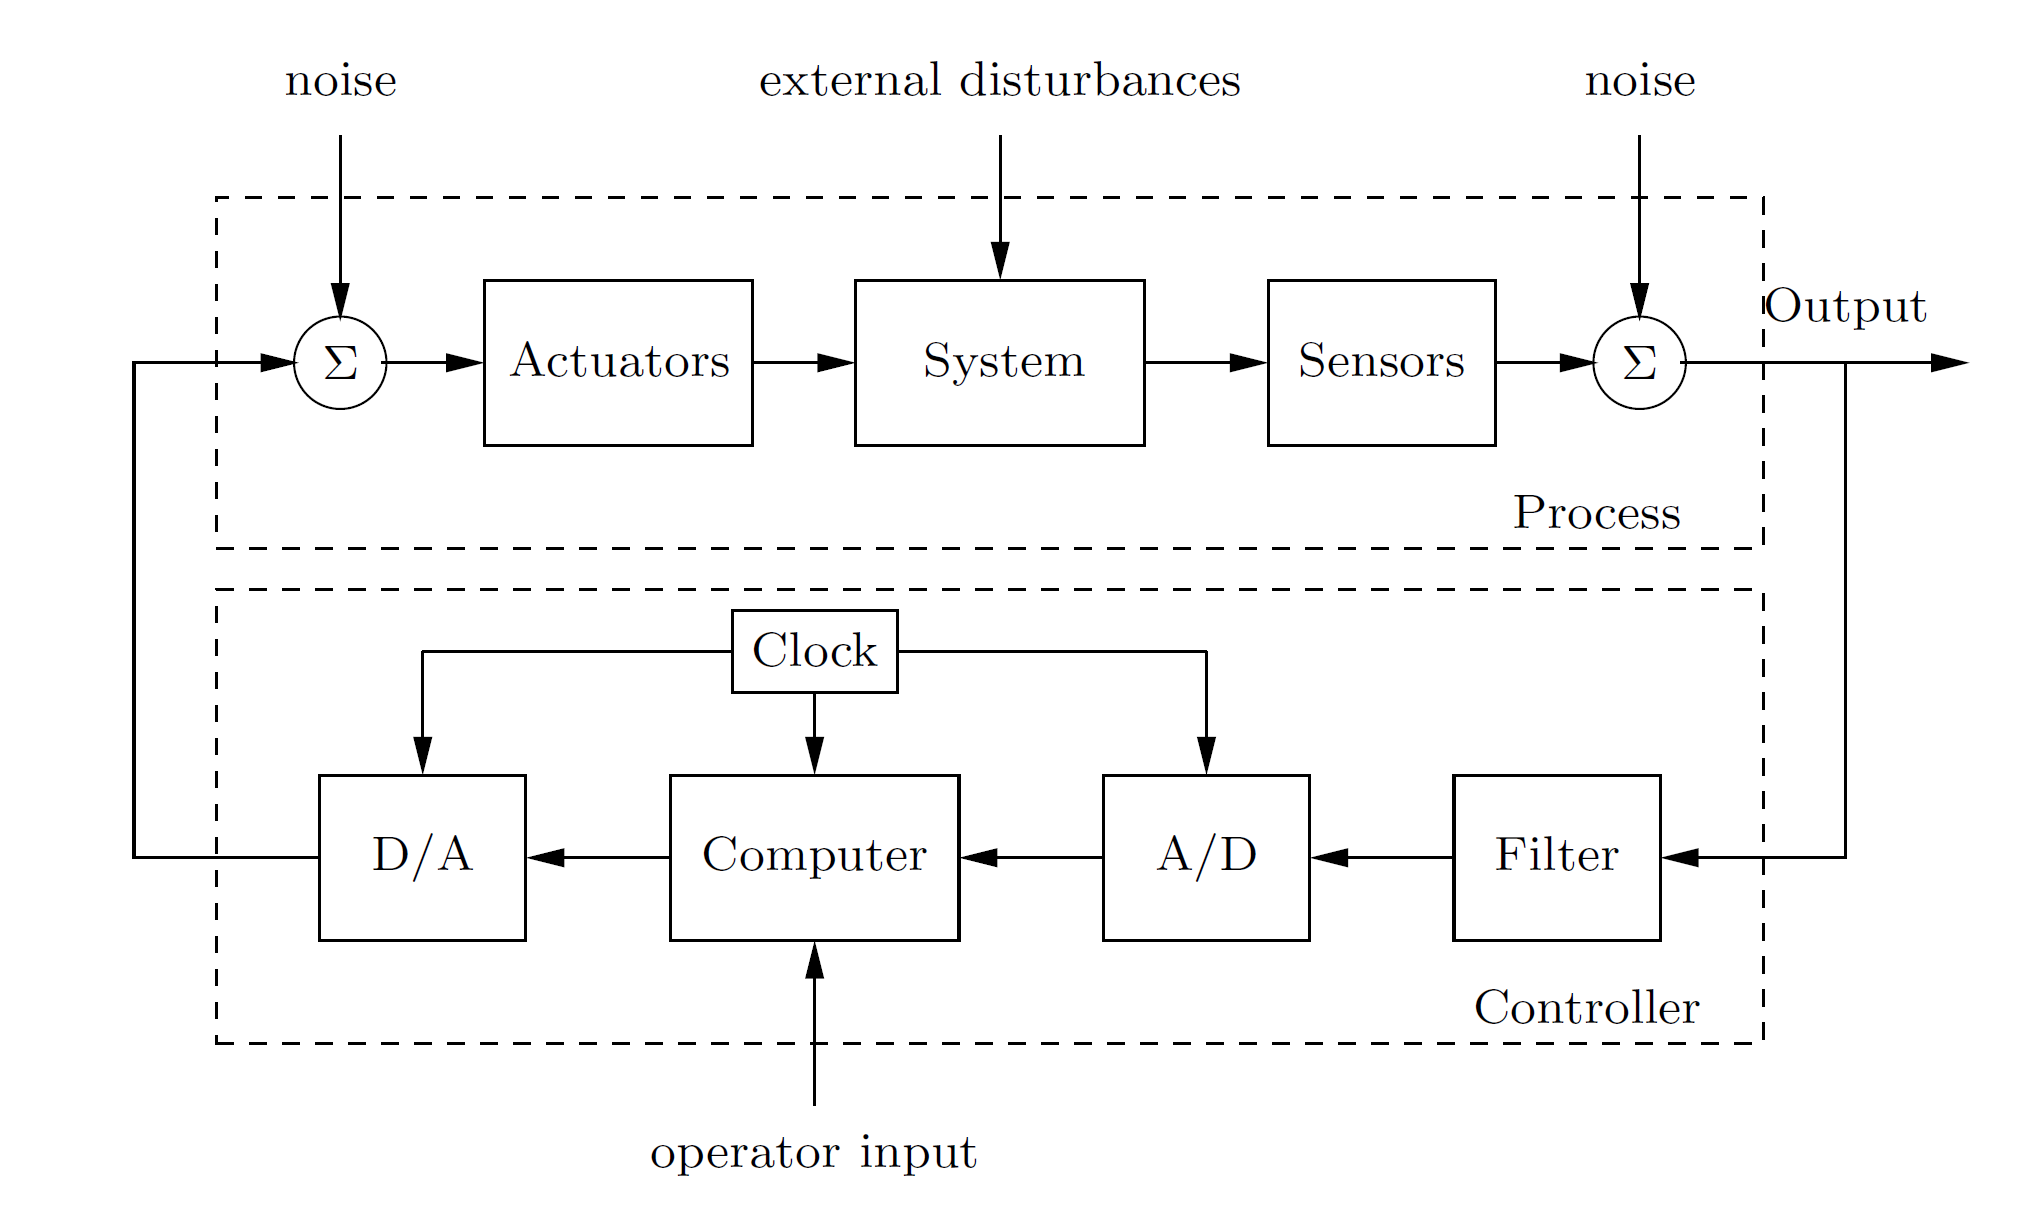
\includegraphics[width = \textwidth]{Full_control_system.png}
\end{column}
\end{columns}

\end{frame}

\begin{frame}
\frametitle{Map of Control theory}
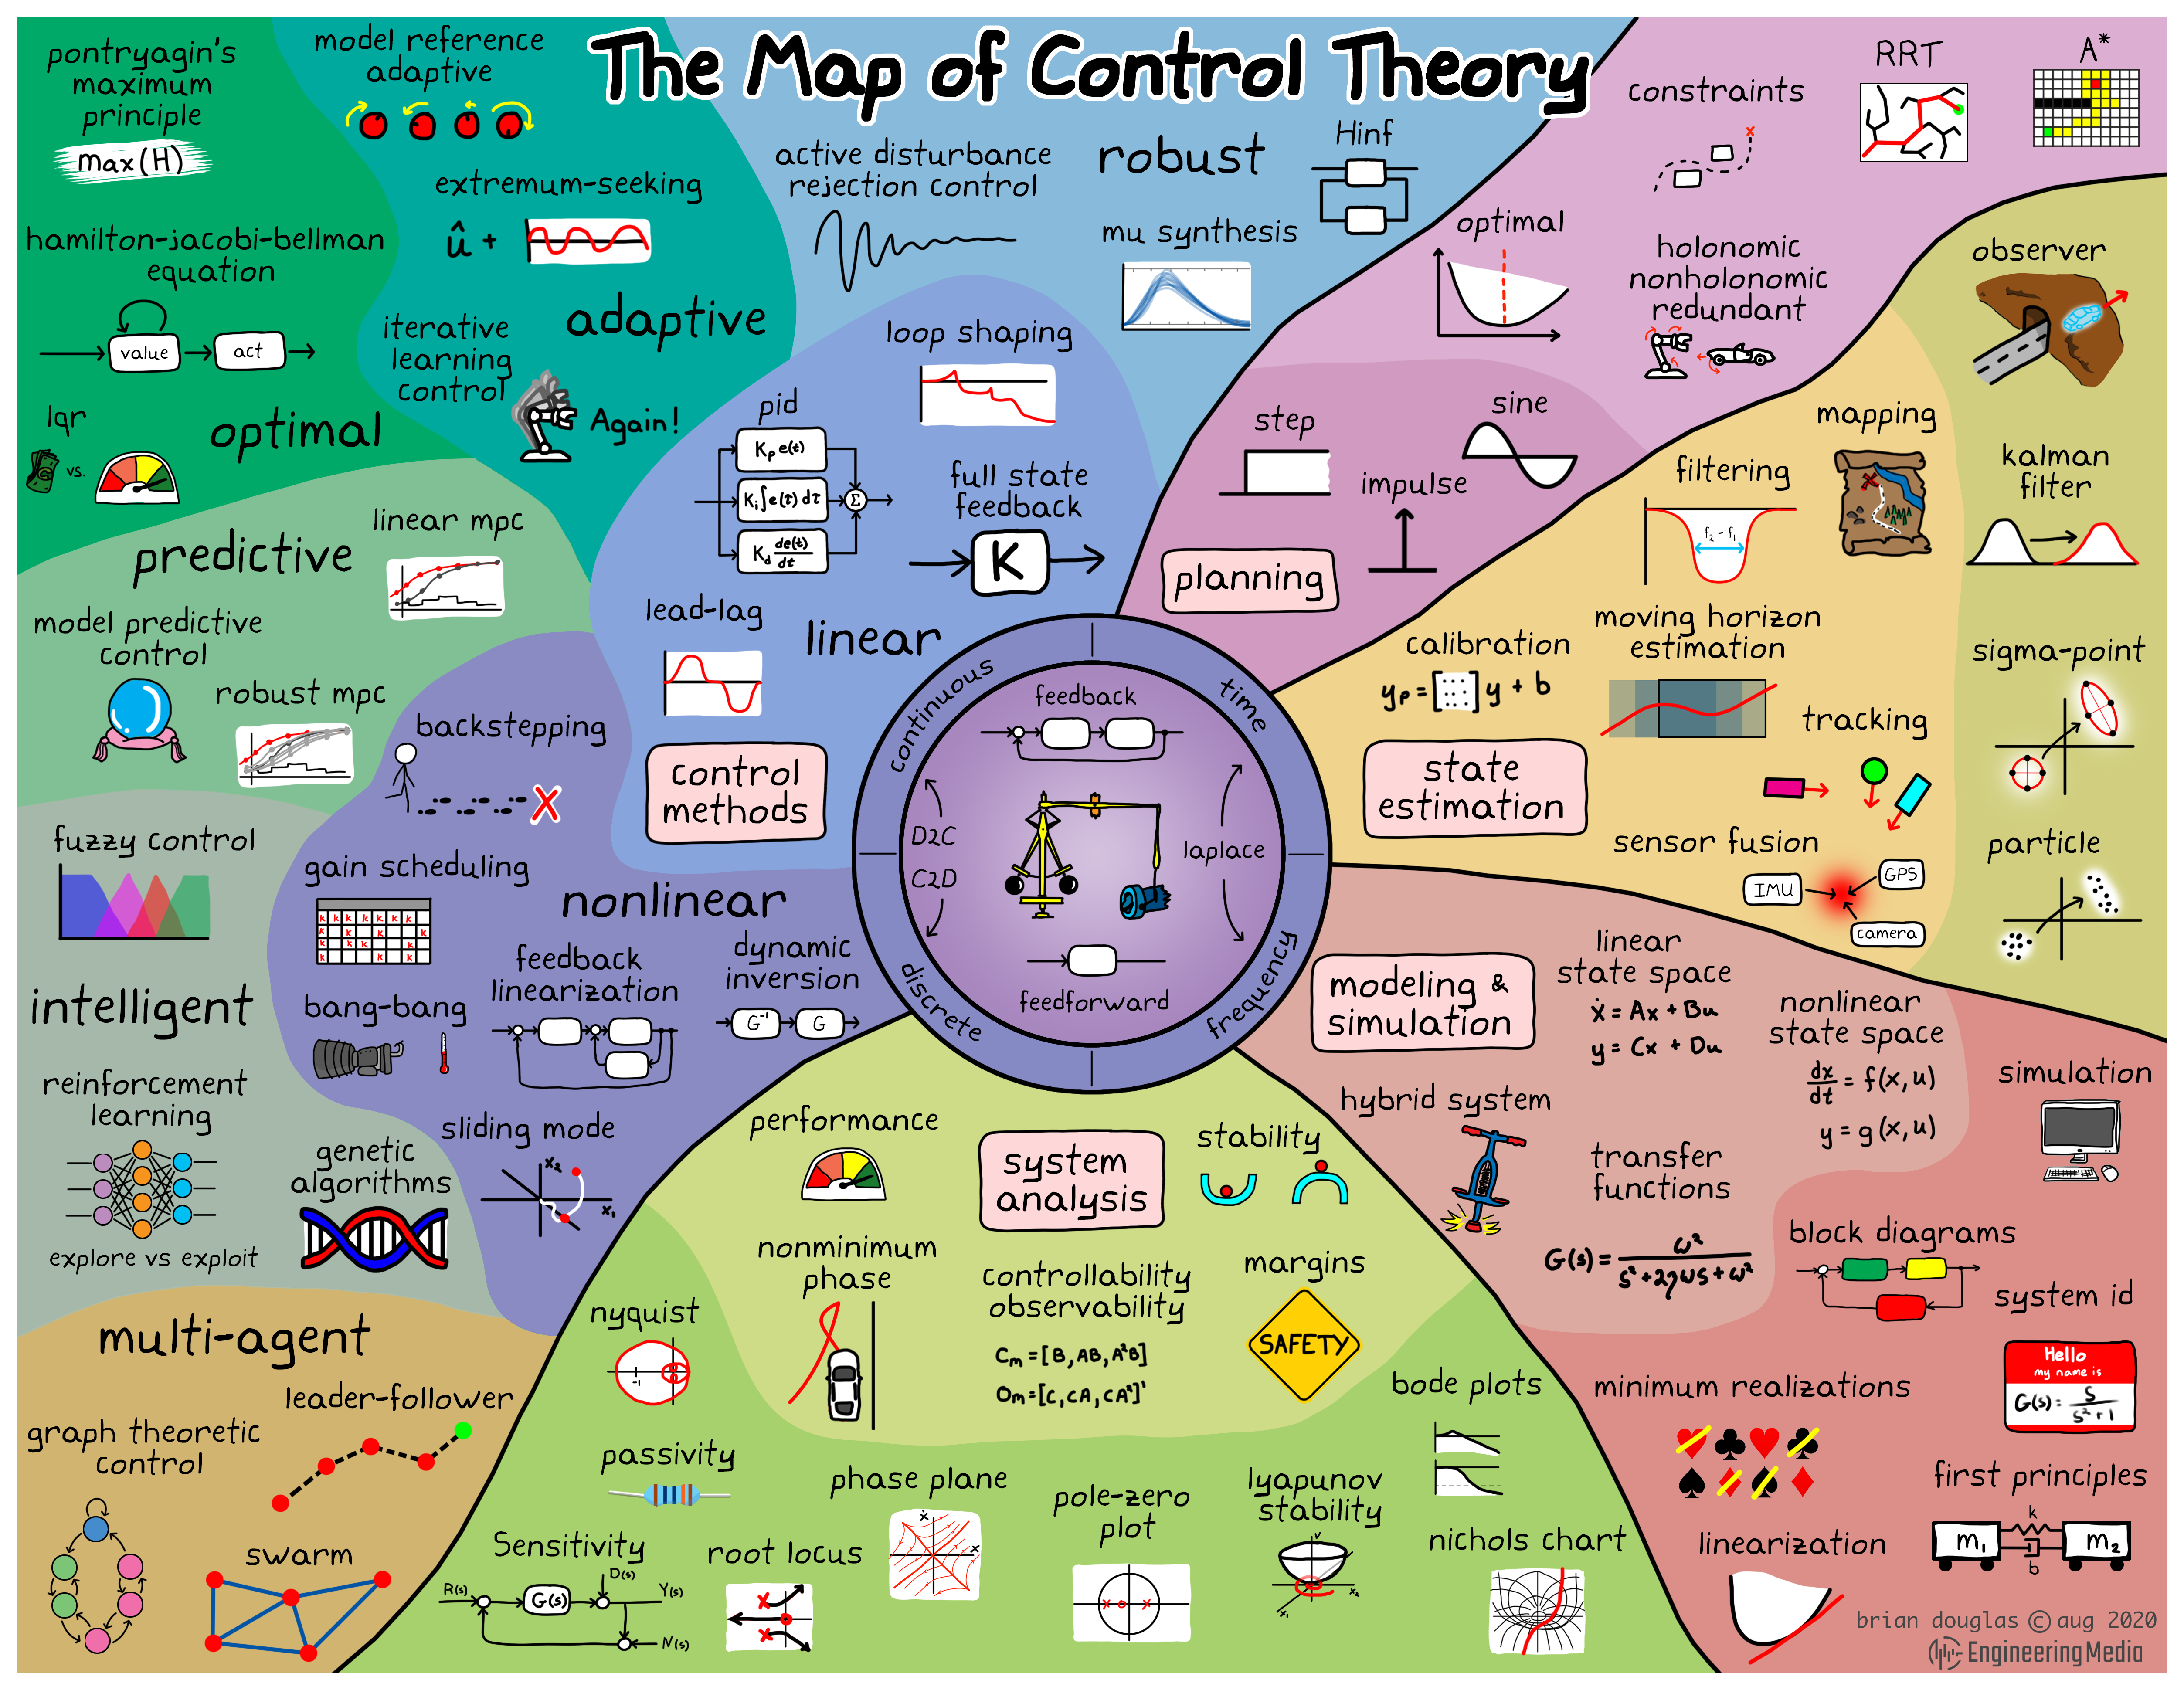
\includegraphics[width = \textwidth]{Control_Map_ver5.png}
\end{frame}

\begin{frame}
\frametitle{What we are going to do}
\begin{itemize}
    \item System modelling - 3DOF model of a thrust vector controlled rocket
    \item Controller design - full state feedback, LQRs
    \item Observer design - linear observer design and Kalman Filters
    \item Simulations in MATLAB Simulink
    \item And more!
\end{itemize}
\end{frame}

\begin{frame}
\frametitle{Further Resources: Links!}
\begin{itemize}
    \item Astrom and Murray's textbook: \href{https://www.cds.caltech.edu/~murray/books/AM08/pdf/fbs-public_24Jul2020.pdf}{Feedback Systems PDF} - Great introduction to linear control theory and frequency domain methods
    \item Brian Douglas's Youtube Channel: \href{https://www.youtube.com/@BrianBDouglas}{Brian Douglas}
    \item Steve Brunton's Youtube Channel: \href{https://www.youtube.com/@Eigensteve}{Steve Brunton}
    \item Journals: IFAC, IEEE, automatica
    \item Podcast: \href{https://www.incontrolpodcast.com/}{InControl}
    \item Many, many, many textbooks
\end{itemize}
\end{frame}

\end{document}